\documentclass[ignorenonframetext,]{beamer}
\setbeamertemplate{caption}[numbered]
\setbeamertemplate{caption label separator}{: }
\setbeamercolor{caption name}{fg=normal text.fg}
\beamertemplatenavigationsymbolsempty
\usepackage{lmodern}
\usepackage{amssymb,amsmath}
\usepackage{ifxetex,ifluatex}
\usepackage{fixltx2e} % provides \textsubscript
\ifnum 0\ifxetex 1\fi\ifluatex 1\fi=0 % if pdftex
  \usepackage[T1]{fontenc}
  \usepackage[utf8]{inputenc}
\else % if luatex or xelatex
  \ifxetex
    \usepackage{mathspec}
  \else
    \usepackage{fontspec}
  \fi
  \defaultfontfeatures{Ligatures=TeX,Scale=MatchLowercase}
\fi
% use upquote if available, for straight quotes in verbatim environments
\IfFileExists{upquote.sty}{\usepackage{upquote}}{}
% use microtype if available
\IfFileExists{microtype.sty}{%
\usepackage{microtype}
\UseMicrotypeSet[protrusion]{basicmath} % disable protrusion for tt fonts
}{}
\newif\ifbibliography
\hypersetup{
            pdftitle={Build to deliver},
            pdfauthor={Galileu Kim},
            pdfborder={0 0 0},
            breaklinks=true}
\urlstyle{same}  % don't use monospace font for urls

% Prevent slide breaks in the middle of a paragraph:
\widowpenalties 1 10000
\raggedbottom

\AtBeginPart{
  \let\insertpartnumber\relax
  \let\partname\relax
  \frame{\partpage}
}
\AtBeginSection{
  \ifbibliography
  \else
    \let\insertsectionnumber\relax
    \let\sectionname\relax
    \frame{\sectionpage}
  \fi
}
\AtBeginSubsection{
  \let\insertsubsectionnumber\relax
  \let\subsectionname\relax
  \frame{\subsectionpage}
}

\setlength{\parindent}{0pt}
\setlength{\parskip}{6pt plus 2pt minus 1pt}
\setlength{\emergencystretch}{3em}  % prevent overfull lines
\providecommand{\tightlist}{%
  \setlength{\itemsep}{0pt}\setlength{\parskip}{0pt}}
\setcounter{secnumdepth}{0}
\usetheme{Madrid}

% packages
\usepackage{attachfile}
\useoutertheme{miniframes} % Alternatively: miniframes, infolines, split
\useinnertheme{circles}

\definecolor{princeton}{rgb}{1.0, 0.6, 0.2}% princeton (primary)
\definecolor{arsenic}{rgb}{0.23, 0.27, 0.29}

\setbeamercolor{palette primary}{bg=princeton,fg=black}
\setbeamercolor{palette secondary}{bg=princeton,fg=black}
\setbeamercolor{palette tertiary}{bg=princeton,fg=black}
\setbeamercolor{palette quaternary}{bg=princeton,fg=black}
\setbeamercolor{structure}{fg=princeton} % itemize, enumerate, etc
\setbeamercolor{section in toc}{fg=princeton} % TOC sections
\setbeamerfont{subtitle}{size=\small}

% override palette coloring with secondary
\setbeamercolor{subsection in head/foot}{bg=arsenic,fg=white}

% defining font
\usepackage[sfdefault]{FiraSans} %% option 'sfdefault' activates Fira Sans as the default text font
\usepackage[T1]{fontenc}
\usepackage{ragged2e}
\renewcommand*\oldstylenums[1]{{\firaoldstyle #1}}

\apptocmd{\frame}{}{\justifying}{} % Allow optional arguments after frame.

% set margins
\setbeamersize{text margin left=12mm,text margin right=12mm}

\title{Build to deliver}
\subtitle{Public services and the politics of administration}
\author{Galileu Kim}
\institute{Princeton University}
\date{November 28, 2017}

\begin{document}
\frame{\titlepage}

\begin{frame}{Overview:}

\begin{itemize}[<+->]
\tightlist
\item
  Motivation.
\item
  The case: Brazil.
\item
  Research question.
\item
  Extant literature and theoretical debate.
\item
  \textcolor{gray}{Results.} (work in progress)
\item
  Conclusion and next steps.
\end{itemize}

\end{frame}

\begin{frame}{It all began\ldots{}}

\center

\begin{center}\includegraphics[width=260px]{health_agents} \end{center}

\end{frame}

\begin{frame}{\ldots{}in Peru.}

\begin{itemize}[<+->]
\tightlist
\item
  A journey to municipalities in the Andes.

  \begin{itemize}[<+->]
  \tightlist
  \item
    Nurses \(\rightarrow\) healthcare.
  \item
    Teachers \(\rightarrow\) education.
  \end{itemize}
\item
  Local service delivery.

  \begin{itemize}[<+->]
  \tightlist
  \item
    Public services as administration.
  \item
    Politics of administration.
  \end{itemize}
\end{itemize}

\end{frame}

\begin{frame}{Across the world:}

\begin{itemize}[<+->]
\tightlist
\item
  Local service delivery is global.

  \begin{itemize}[<+->]
  \tightlist
  \item
    Decentralization in developing and developed world.

    \begin{itemize}[<+->]
    \tightlist
    \item
      \textcolor{gray}{Falleti 2010, Ferwerda 2015.}
    \end{itemize}
  \item
    Delegation to local governments.

    \begin{itemize}[<+->]
    \tightlist
    \item
      \textcolor{gray}{Ahmad and Brosio 2008.}
    \end{itemize}
  \item
    Restructuring of public services delivery.

    \begin{itemize}[<+->]
    \tightlist
    \item
      \textcolor{gray}{OECD 2016.}
    \end{itemize}
  \end{itemize}
\end{itemize}

\end{frame}

\begin{frame}{Delegation in the world:}

\begin{center}\includegraphics[width=290px]{map_share} \end{center}

\end{frame}

\begin{frame}{Welfare implications:}

\begin{center}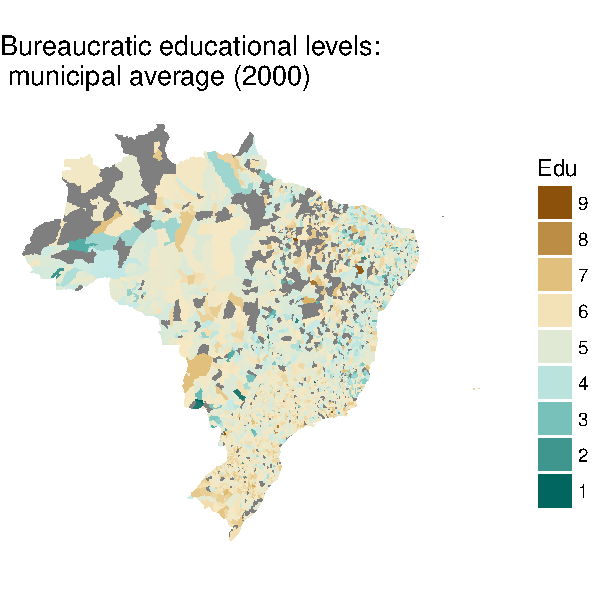
\includegraphics[width=280px]{presentation_cp_files/figure-beamer/unnamed-chunk-3-1} \end{center}

\end{frame}

\begin{frame}{Case study:}

\begin{itemize}[<+->]
\tightlist
\item
  Brazil.

  \begin{itemize}[<+->]
  \tightlist
  \item
    Primary education and healthcare under municipal jurisdiction.

    \begin{itemize}[<+->]
    \tightlist
    \item
      \textcolor{gray}{Arretche 2016.}
    \end{itemize}
  \item
    Municipal autonomy over hiring decisions.

    \begin{itemize}[<+->]
    \tightlist
    \item
      \textcolor{gray}{Pessoa 1988.}
    \end{itemize}
  \item
    Unique dataset of all municipal bureaucrats from 1984-2015.

    \begin{itemize}[<+->]
    \tightlist
    \item
      RAIS (Annual Report of Social Information).
    \end{itemize}
  \end{itemize}
\end{itemize}

\end{frame}

\begin{frame}{Expenditure, local share:}

\begin{center}\includegraphics{presentation_cp_files/figure-beamer/unnamed-chunk-4-1} \end{center}

\end{frame}

\begin{frame}{Personnel, local share:}

\begin{center}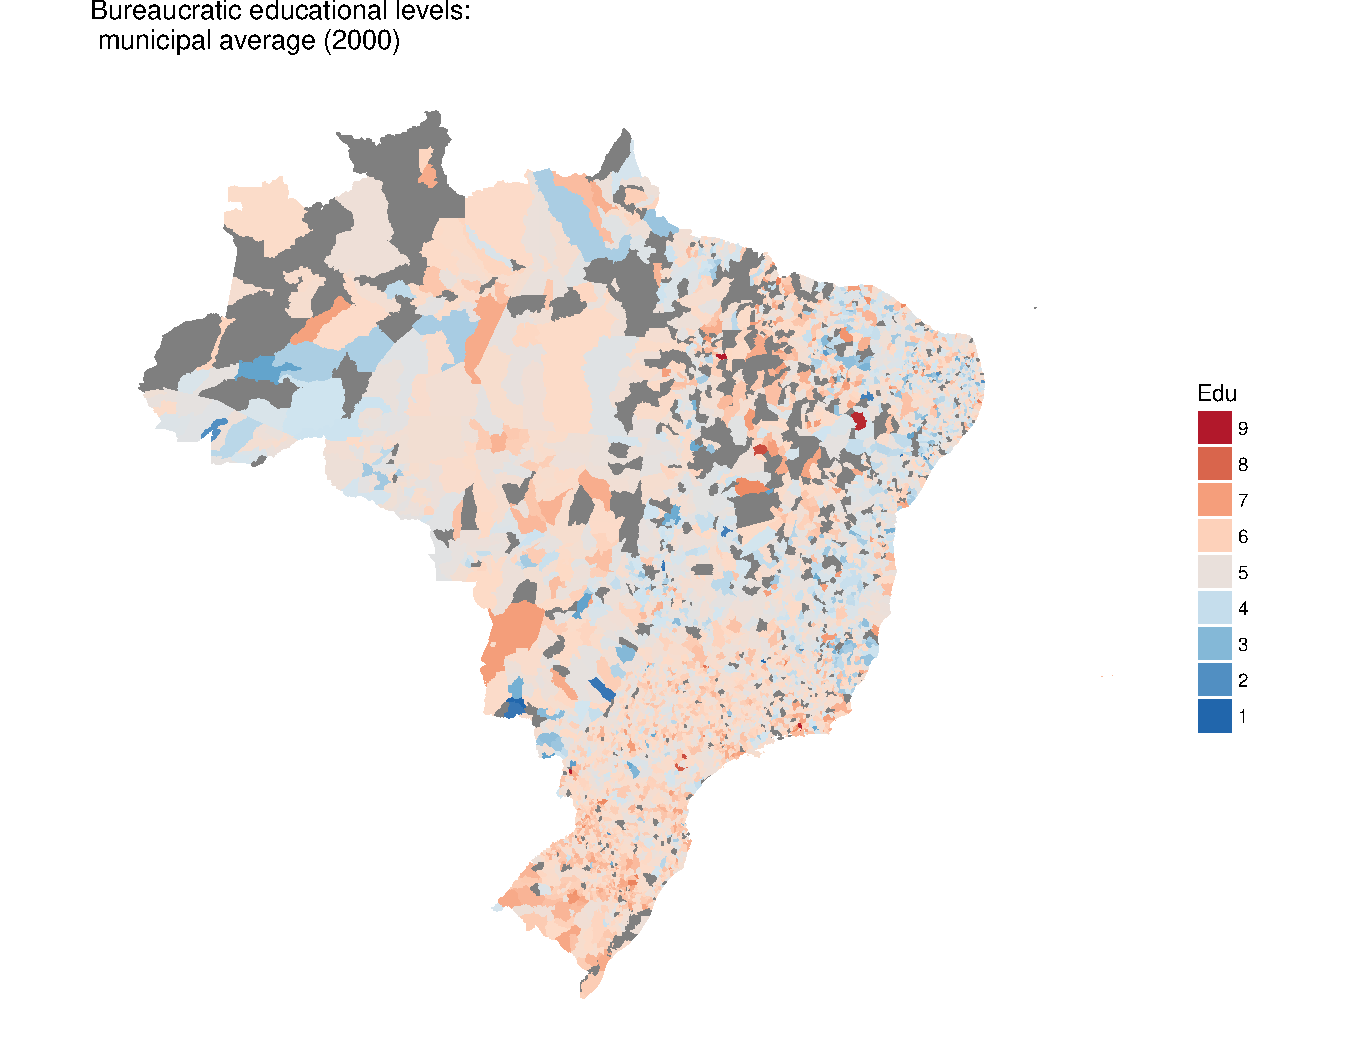
\includegraphics{presentation_cp_files/figure-beamer/unnamed-chunk-5-1} \end{center}

\end{frame}

\begin{frame}{Map of Teachers:}

\begin{center}\includegraphics[width=185px]{map_teacher} \end{center}

\end{frame}

\begin{frame}{Research question:}

\center

\begin{center}\includegraphics[width=270px]{dag} \end{center}

\justifying

\begin{itemize}[<+->]
\tightlist
\item
  Under what conditions do local politicians hire competent bureaucrats
  to deliver public services?

  \begin{itemize}[<+->]
  \tightlist
  \item
    Intersection of politics and public administration.

    \begin{itemize}[<+->]
    \tightlist
    \item
      \textcolor{gray}{Tendler 1997, Geddes 1994.}
    \end{itemize}
  \item
    Two public services:

    \begin{itemize}[<+->]
    \tightlist
    \item
      Education (teachers).
    \item
      Healthcare (doctors and nurses).
    \end{itemize}
  \end{itemize}
\end{itemize}

\end{frame}

\begin{frame}{Extant Literature:}

\begin{itemize}[<+->]
\tightlist
\item
  Three strands of literature.

  \begin{itemize}[<+->]
  \tightlist
  \item
    State capacity.
  \item
    Developmental state and bureaucracies.
  \item
    Clientelism/patronage.
  \end{itemize}
\end{itemize}

\end{frame}

\begin{frame}{State capacity:}

\begin{itemize}[<+->]
\tightlist
\item
  What is the state capable of?

  \begin{itemize}[<+->]
  \tightlist
  \item
    Taxation, industrialization, neither.

    \begin{itemize}[<+->]
    \tightlist
    \item
      \textcolor{gray}{Tilly 1994, Kohli 2004, Van de Walle 2001.}
    \end{itemize}
  \end{itemize}
\item
  State \(\rightarrow\) local states.

  \begin{itemize}[<+->]
  \tightlist
  \item
    Weberian state decentralized.

    \begin{itemize}[<+->]
    \tightlist
    \item
      \textcolor{gray}{Falleti 2010, Eaton 2004.}
    \end{itemize}
  \end{itemize}
\item
  State capacity \(\rightarrow\) capacities.

  \begin{itemize}[<+->]
  \tightlist
  \item
    Multiplication of roles.

    \begin{itemize}[<+->]
    \tightlist
    \item
      \textcolor{gray}{Skocpol 1985, Soifer 2008, Centeno et al. 2017.}
    \end{itemize}
  \end{itemize}
\end{itemize}

\end{frame}

\begin{frame}{Developmental state and bureaucracy:}

\begin{itemize}[<+->]
\tightlist
\item
  Variation in state capacity.

  \begin{itemize}[<+->]
  \tightlist
  \item
    Bureaucracy \(\rightarrow\) economic development.

    \begin{itemize}[<+->]
    \tightlist
    \item
      \textcolor{gray}{Johnson 1982, Evans 1995, Kohli 2004.}
    \end{itemize}
  \item
    Institutional characteristics.

    \begin{itemize}[<+->]
    \tightlist
    \item
      Educated, meritocratic, depoliticized.
    \end{itemize}
  \end{itemize}
\item
  Political entrepreneurship and change over time.

  \begin{itemize}[<+->]
  \tightlist
  \item
    Reassess Weber's wall of separation.

    \begin{itemize}[<+->]
    \tightlist
    \item
      \textcolor{gray}{Grindle 2012, Geddes 1994.}
    \end{itemize}
  \item
    Ideal type \(\rightarrow\) changing institutions.

    \begin{itemize}[<+->]
    \tightlist
    \item
      \textcolor{gray}{Thelen 1999, Tendler 1997.}
    \end{itemize}
  \end{itemize}
\end{itemize}

\end{frame}

\begin{frame}{Clientelism and patronage:}

\begin{itemize}[<+->]
\tightlist
\item
  Political motivation behind goods allocation.

  \begin{itemize}[<+->]
  \tightlist
  \item
    Politicians (and voters) as strategic actors.

    \begin{itemize}[<+->]
    \tightlist
    \item
      \textcolor{gray}{Stokes 2005, Stokes et al. 2015, Diaz-Cayeros et al. 2017}
    \end{itemize}
  \end{itemize}
\item
  Patronage as clientelistic redistribution.

  \begin{itemize}[<+->]
  \tightlist
  \item
    Public jobs to loyalists or party members.

    \begin{itemize}[<+->]
    \tightlist
    \item
      \textcolor{gray}{Calvo and Murillo 2004, Hagopian 1997, Grindle 2012.}
    \end{itemize}
  \end{itemize}
\item
  Patronage refined.

  \begin{itemize}[<+->]
  \tightlist
  \item
    Who gets hired?
  \item
    What qualifications?
  \end{itemize}
\end{itemize}

\end{frame}

\begin{frame}{Build to deliver:}

\begin{itemize}[<+->]
\tightlist
\item
  Politicians decide who to hire, retain or fire.

  \begin{itemize}[<+->]
  \tightlist
  \item
    Education level.
  \item
    Type of contract (permanent or temporary).
  \item
    Wage.
  \item
    Work experience (years).
  \end{itemize}
\item
  Possible mechanisms:

  \begin{itemize}[<+->]
  \tightlist
  \item
    Economic modernization.
  \item
    State-society synergy.

    \begin{itemize}[<+->]
    \tightlist
    \item
      \textcolor{gray}{Evans 1996}
    \end{itemize}
  \item
    Party turnover (time horizon).

    \begin{itemize}[<+->]
    \tightlist
    \item
      \textcolor{gray}{Akhtari et al. 2017.}
    \end{itemize}
  \item
    Overlapping jurisdiction.

    \begin{itemize}[<+->]
    \tightlist
    \item
      \textcolor{gray}{Gulzaar and Pasquale 2017.}
    \end{itemize}
  \end{itemize}
\end{itemize}

\end{frame}

\begin{frame}{Results (work in progress):}

\begin{itemize}[<+->]
\tightlist
\item
  Data collection effort.

  \begin{itemize}[<+->]
  \tightlist
  \item
    Demographic census.

    \begin{itemize}[<+->]
    \tightlist
    \item
      Municipal level, 1980-2010.
    \end{itemize}
  \item
    Municipal budget.

    \begin{itemize}[<+->]
    \tightlist
    \item
      Breakdown by function, 1998-2010.
    \end{itemize}
  \item
    Electoral data.

    \begin{itemize}[<+->]
    \tightlist
    \item
      Mayoral elections from 1994 to 2014.
    \end{itemize}
  \item
    Education and healthcare infrastructure.

    \begin{itemize}[<+->]
    \tightlist
    \item
      Unique Health System (SUS).
    \item
      School census.
    \end{itemize}
  \end{itemize}
\end{itemize}

\end{frame}

\begin{frame}{Conclusion:}

\begin{itemize}[<+->]
\tightlist
\item
  Public service as administration.

  \begin{itemize}[<+->]
  \tightlist
  \item
    Bureaucratic organization behind delivery.
  \end{itemize}
\item
  Going local.

  \begin{itemize}[<+->]
  \tightlist
  \item
    Municipal governments and capacities.
  \item
    Executive leadership and personnel.
  \end{itemize}
\item
  Build to deliver.

  \begin{itemize}[<+->]
  \tightlist
  \item
    Why do politicians build competent bureaucracies?
  \end{itemize}
\end{itemize}

\end{frame}

\begin{frame}{Next steps:}

\begin{itemize}[<+->]
\tightlist
\item
  From framing to testing:

  \begin{itemize}[<+->]
  \tightlist
  \item
    Data gathering effort largely concluded.
  \item
    Descriptive and causal analysis ongoing.
  \end{itemize}
\item
  Incorporating qualitative evidence.

  \begin{itemize}[<+->]
  \tightlist
  \item
    Fieldwork in Brazil.
  \item
    Explore accounts of local administrative changes.
  \item
    Motivations and decision-making process.
  \end{itemize}
\end{itemize}

\end{frame}

\begin{frame}{Thank you!}

\begin{itemize}[<+->]
\tightlist
\item
  Please send comments to
  \fontfamily{cmtt}\selectfont \href{mailto:galileuk@princeton.edu}{\nolinkurl{galileuk@princeton.edu}}.
\end{itemize}

\end{frame}

\end{document}
